\documentclass{beamer}
\usepackage[utf8]{inputenc}
\usepackage[T1]{fontenc}
\usepackage{mathabx}
\usepackage{mathpazo}
\usepackage{eulervm}
\usepackage{natbib}
\usepackage{enumerate}
\usepackage{mathrsfs}

\usetheme{Madrid}
\usefonttheme{structurebold}
\usecolortheme{dove}
\title{VE401 RC Week5}
\author{Wang Yangyang}
\date{2022 Spring}
\institute{UM-SJTU JI}
\setbeamersize{text margin left = 20pt, text margin right = 20pt}

\AtEndDocument{\begin{frame}{End}

                  Credit to Zhanpeng Zhou (TA of SP21)
                  
                  Credit to Fan Zhang (TA of SU21)
                  
                  Credit to Liying Han (TA of SP21)
                  
                  Credit to Zhenghao Gu (TA of SP20)
               \end{frame}}
                
\definecolor{antiquefuchsia}{rgb}{0.57, 0.36, 0.51}
\newcommand{\bb}[1]{\textcolor{antiquefuchsia}{\textbf{\textit{#1}}}}

\begin{document}
\maketitle

\begin{frame}
\frametitle{Outline}
\tableofcontents
\end{frame}

%\AtBeginSection[ ]
%{
%\begin{frame}{Outline for \secname}
%	\tableofcontents[currentsection, hideothersubsections, %sectionstyle=show/show]
%\end{frame}
%}

\AtBeginSubsection[]{
  \frame<beamer>{ 
    \frametitle{Outline}   
    \tableofcontents[currentsection,currentsubsection] 
  }
}

\section{Reliability}
\subsection{Reliability and Hazard}
\begin{frame}{Reliability}
\begin{block}{Definition}
Suppose a unit $A$ fails \bb{randomly}, and we describe the time it fails by the continuous random variable $T_{A}$.

The density of $T_{A}$ is called the \bb{failure density} $f_{A}$.
The cumulative distribution function of $T_{A}$ is denoted by $F_{A}$.
We note that
$$
\begin{aligned}
f_{A}(t) &=\lim _{\Delta t \rightarrow 0} \frac{P[t \leq T \leq t+\Delta t]}{\Delta t} \\
&=\lim _{\Delta t \rightarrow 0} \frac{F_{A}(t+\Delta t)-F_{A}(t)}{\Delta t}
\end{aligned}
$$

The \bb{reliability function} $R_{A}$ gives the probability that $A$ is working at time $t \geq 0$
$$
\begin{aligned}
R_{A}(0) &=1 \\
R_{A}(t) &=1-P[\text { component A fails before time } t] \\
&=1-F_{A}(t)
\end{aligned}
$$
\end{block}
\end{frame}

\begin{frame}{Hazard}
\begin{block}{Definition}
\bb{Hazard rate} $\varrho_{A}$ defined by
$$
\begin{aligned}
\varrho_{A}(t) &=\lim _{\Delta t \rightarrow 0} \frac{P[t \leq T \leq t+\Delta t \mid t \leq T]}{\Delta t} \\
&=\lim _{\Delta t \rightarrow 0} \frac{P[t \leq T \leq t+\Delta t]}{P[T \geq t] \cdot \Delta t}=\frac{f_{A}(t)}{R_{A}(t)}
\end{aligned}
$$
\end{block}
\begin{block}{Interpretation}
\begin{itemize}
\item If $\varrho$ is decreasing, then as time goes by a failure is more likely to occur earlier in the time interval.
\item If $\varrho$ is steady, a failure tends to occur during this period due mainly to random factors.
\item If $\varrho$ is increasing, then as time goes by a failure is more likely to occur.
\end{itemize}
\end{block}
\end{frame}

\begin{frame}{Hazard}
\begin{block}{Theorem}
Let $X$ be a random variable with \bb{failure density} $f$, \bb{reliability function} $R$, and \bb{hazard rate} $\varrho$. Then
$$
R(t)=e^{-\int_{0}^{t} \varrho(x) d x}
$$
\end{block}
\begin{block}{Proof}
Proof.
Since $R(x)=1-F(x)$ we have $R^{\prime}(x)=-F^{\prime}(x)$. Therefore,
$$
\varrho(x)=\frac{f(x)}{R(x)}=\frac{F^{\prime}(x)}{R(x)}=-\frac{R^{\prime}(x)}{R(x)}
$$
$$
R^{\prime}(x)=-\rho(x) R(x)
$$
Solving this equation with $R(0)=1$ (because A is always working at the beginning), we obtain the result.
\end{block}
\end{frame}


\begin{frame}{Exponential Distribution}
\begin{itemize}
\item Density function. $\beta>0$ is a parameter,
$$
f(x)= \begin{cases}\beta e^{-\beta x}, & x>0 \\ 0, & \text { otherwise. }\end{cases}
$$
\item Mean.
$$
\mu=\frac{1}{\beta}
$$
\item Variance.
$$
\sigma^{2}=\frac{1}{\beta^{2}}
$$
\item Reliability features.
$$
\rho(t)=\beta$$$$R(t)=e^{-\beta t}, f(t)=\rho(t) R(t)=\beta e^{-\beta t} .
$$
\end{itemize}
\end{frame}

\begin{frame}{Weibull Distribution}
\begin{itemize}
\item Density function. $\alpha, \beta>0$ are parameters,
$$
f(x)= \begin{cases}\alpha \beta x^{\beta-1} e^{-\alpha x^{\beta}}, & x>0 \\ 0, & \text { otherwise }\end{cases}
$$
\item Mean.
$$
\mu=\alpha^{-1 / \beta} \Gamma(1+1 / \beta)
$$
\item Variance.
$$
\sigma^{2}=\alpha^{-2 / \beta} \Gamma(1+2 / \beta)-\mu^{2}
$$
\item Reliability features.
$$
\rho(t)=\alpha \beta t^{\beta-1}$$$$ R(t)=e^{-\alpha t^{\beta}}, f(t)=\rho(t) R(t)=\alpha \beta t^{\beta-1} e^{-\alpha t^{\beta}}
$$
\end{itemize}
\end{frame}

\subsection{System}
\begin{frame}{System}
$R_{i}$ is the reliability of the ith component, then
\begin{enumerate}
\item reliability of a series system with $k$ components
$$
R_{s}(t)=\prod_{i=1}^{k} R_{i}(t)
$$
\item reliability of a parallel system with $k$ components
$$R_{p}(t)=1-P\text{[all components fail before t]}=1-\prod_{i=1}^{k}\left(1-R_{i}(t)\right)$$
\end{enumerate}
\end{frame}


\section{Basic Statistics}
\subsection{Samples and Data}
\begin{frame}{Sample and Percentile}
\begin{block}{Definition}
A \bb{random sample} of size $n$ from the distribution of $X$ is a collection of $n$ independent random variables $X_{1}, \ldots, X_{n}$, each with the same distribution as $X$.
\begin{itemize}
\item i.i.d random variables
\item Sample size $n$ should neither be too small or large, usually smaller than $5 \%$ of the population.
\end{itemize}

\bb{Percentiles}: The $x$ th percentile is defined as the value $d_{x}$ of the data such that $x \%$ of the values of the data are less than or equal to $d_{x}$.
\end{block}
\end{frame}

\begin{frame}{Quantile}
\begin{block}{Definition}
\bb{Quartiles}:(special cases of percentiles)
\begin{itemize}
\item $25 \%$ of the data are no greater than the first quartile $q_{1}$.
\item $50 \%$ are no greater than the second quartile $q_{2}$ (median).
\item $75 \%$ are no greater than the third quartile $q_{3}$.
\end{itemize}
\end{block}
\begin{block}{Definition}
\bb{Interquartile Range}: $\mathrm{IQR}=q_{3}-q_{1}$.
\begin{itemize}
\item Median describes location of data.
\item IQR describes dispersion of data.
\end{itemize}
\end{block}
\end{frame}

\begin{frame}{Calculating Quartiles}

Suppose that our list of $n$ data has been ordered from smallest to largest, so that
$$
x_{1} \leq x_{2} \leq x_{3} \leq \cdots \leq x_{n}
$$
Then the median $q_{2}$ :
$$
q_{2}= \begin{cases}x_{(n+1) / 2} & \text { if } n \text { is odd } \\ \frac{1}{2}\left(x_{n / 2}+x_{n / 2+1}\right) & \text { if } n \text { is even }\end{cases}
$$
The first quartile $q_{1}$ :
\begin{itemize}
\item the median of the smallest $n / 2$ elements if $n$ is even.
\item the average of the median of the smallest $(n-1) / 2$ elements and the median of the smallest $(n+1) / 2$ elements of the list if $n$ is odd.
\end{itemize}
The third quartile $q_{3}:$ replace "smallest" with "largest" in the above definition.

\end{frame}

\subsection{Data Visualization}
\begin{frame}{Histogram}
\begin{enumerate}
\item Determine \bb{bin width}
\begin{itemize}
\item{Sturges's Rule}
$$
k=\left\lceil\log _{2}(n)\right\rceil+1
,\quad
h=\frac{\max \left\{x_{i}\right\}-\min \left\{x_{i}\right\}}{k}
$$

\item{Freedman-Diaconis Rule}
$$
h=\frac{2 \cdot \mathrm{IQR}}{\sqrt[3]{n}}
$$
\end{itemize}

which should be rounded up to the precision of the data.

\item Determine \bb{the lower boundary}:

Ideally, take the smallest datum, subtract one-half of the smallest decimal of the data and then successively add the bin width to obtain the bins.

In practice, just choosing the lower boundary where \bb{no datum can lie on the boundary} is fine.
\end{enumerate}
\end{frame}

\begin{frame}{Histogram}
\begin{center}
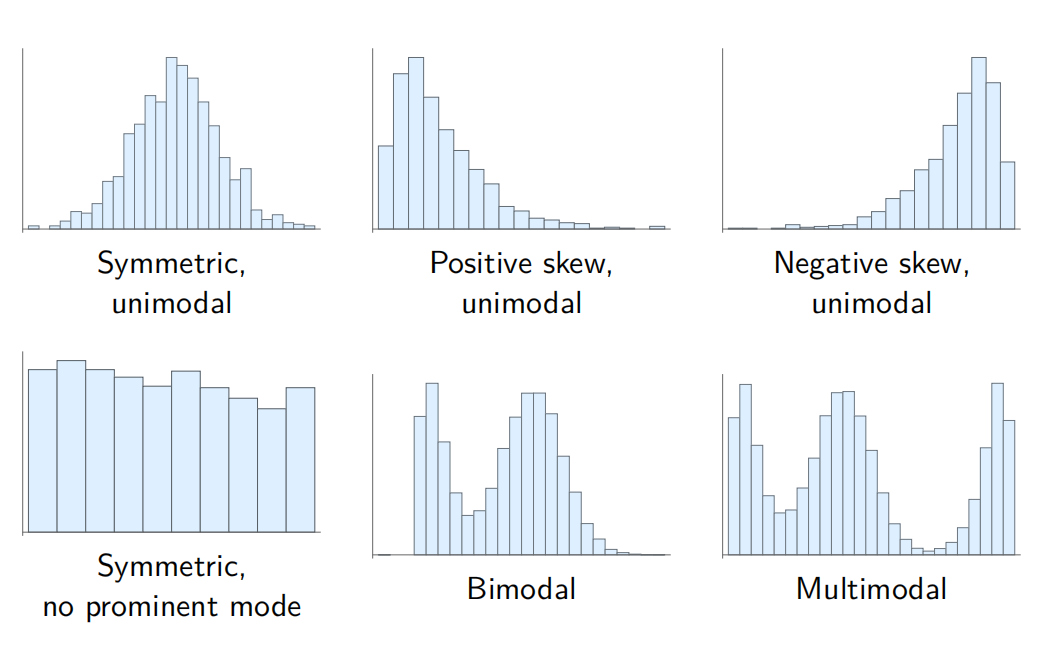
\includegraphics[scale=0.4]{hist.png}
\end{center}
\end{frame}

\begin{frame}{Details and Interpretation}
\begin{center}
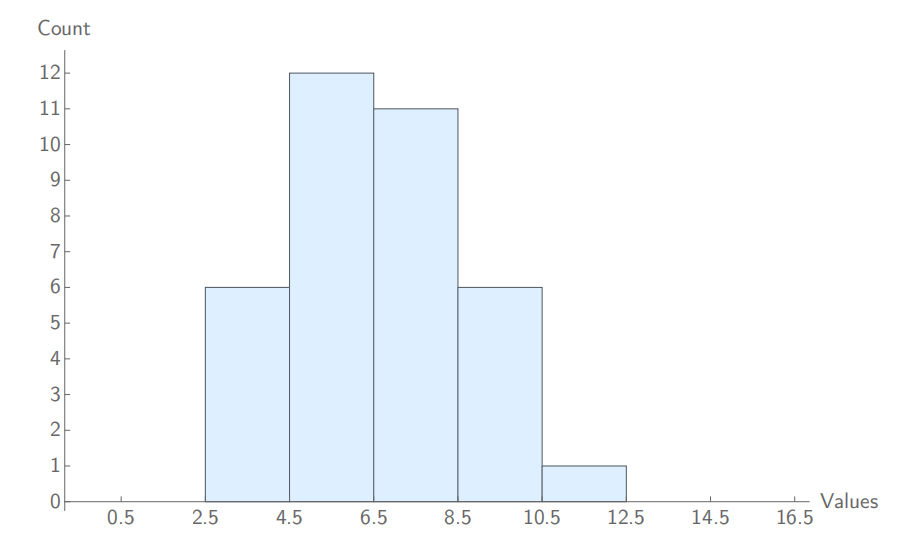
\includegraphics[scale=0.25]{ex1.png}
\end{center}
(1/2) for labelling the axes

(1/2) for starting point that prevents data from falling on the boundary.

(1) is for the general shape and correctness of the histogram.


This histogram has a \bb{unimodal} shape (1/2 Mark) which is consistent with a normal distribution.

It is not significantly \bb{skewed}, (1/2 Mark) again consistent with a normal distribution.

Therefore, there is no evidence that the data does not come from a normal distribution. (1 Mark)
\end{frame}

\begin{frame}{Stem-and-Leaf Diagram}
\begin{enumerate}
\item Choose a convenient number of leading decimal digits to serve as stems,
\item label the rows using the stems,
\item for each datum of the random sample, note down the digit following the stem in the corresponding row,
\item turn the graph on its side to get an impression of its distribution.
\end{enumerate}
\begin{tabular}{r|l} 
Stem & Leaves \\
\hline 0 & 000000011111222222222223333444445555566666777777888899 \\
1 & 00011111223344444455555678899 \\
2 & 223669 \\
3 & 012456 \\
4 & \\
5 & 2 \\
6 & 8
\end{tabular}
\bb{Stem Units}: 100 (Important!)
\end{frame}

\begin{frame}{Box-and-Whisker Plot}
We define the \bb{inner fences}
$$
f_{1}=q_{1}-\frac{3}{2} \mathrm{IQR}, \quad f_{3}=q_{3}+\frac{3}{2} \mathrm{IQR}
$$
The "whiskers" (lines extending to the left and right of the box) end at the adjacent values
$$
a_{1}=\min \left\{x_{k}: x_{k} \geq f_{1}\right\}, \quad a_{3}=\max \left\{x_{k}: x_{k} \leq f_{3}\right\}
$$
We define the \bb{outer fences}
$$
F_{1}=q_{1}-3 \mathrm{IQR}, \quad F_{3}=q_{3}+3 \mathrm{IQR}
$$
Measurements $x_{k}$ that lie outside the inner fences but inside the outer fences are called \bb{near outliers}. 

Those outside the outer fences are known as \bb{far outliers}.
\end{frame}

\begin{frame}{Box-and-Whisker Plot}
\begin{center}
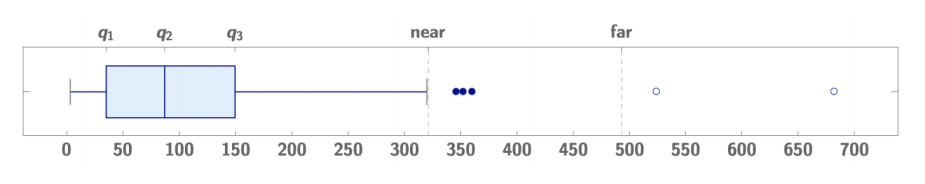
\includegraphics[scale=0.45]{box.png}
\end{center}
\begin{block}{Interpretation}
Interpretation: If data is obtained from a normal distribution, one would expect to see
\begin{itemize}
\item a symmetric median line in the middle of the box;
\item equally long whiskers;
\item very few near outliers and no far outliers.
\end{itemize}
\end{block}
\end{frame}

\begin{frame}{Details and Interpretation}
\begin{center}
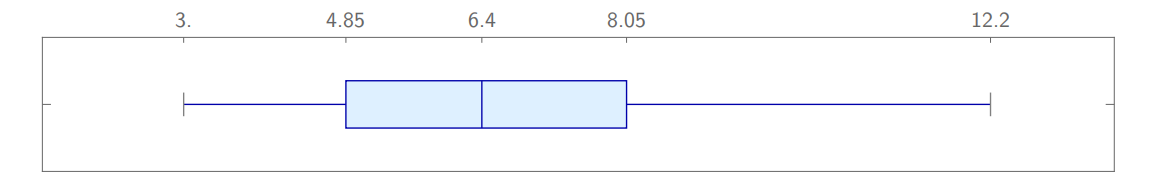
\includegraphics[scale=0.3]{ex2.png}
\end{center}
(1/2) for the general shape of the boxplot,

(1/2) for labelling the ordinate

(1) for the correct drawing indicating the whisker values, $q_{1}, q_{2}, q_{3}$ and for correctly identified outlier(s), if any.


The whiskers are moderately \bb{asymmetric} (1/2)

but the \bb{median line} is not too far from the center of the box (1/2).

There is no \bb{outlier}, (1/2)

and in summary no strong evidence that the data does not come from a normal distribution. (1/2)
\end{frame}

\section{Estimator}
\subsection{Parameter Estimation}
\begin{frame}{Estimation}
\begin{itemize}
\item \bb{Statistic}: a random variable that is derived from $X_{1}, \ldots, X_{n}$.
\item \bb{Estimator}: a statistic that is used to estimate a population parameter.
\item \bb{Point estimate}: a value of the estimator.
\item \bb{Unbiased}: expectation of an estimator $\widehat{\theta}$ is equal to the true parameter.
$$
\mathrm{E}[\widehat{\theta}]=\theta, \quad \text { bias }=\theta-\mathrm{E}[\widehat{\theta}]
$$
\item \bb{Mean square error}.
$$
\begin{aligned}
\operatorname{MSE}(\widehat{\theta}) &=\mathrm{E}\left[(\widehat{\theta}-\theta)^{2}\right] \\
&=\mathrm{E}\left[(\widehat{\theta}-\mathrm{E}[\widehat{\theta}])^{2}\right]+(\theta-\mathrm{E}[\widehat{\theta}])^{2} \\
&=\operatorname{Var}[\widehat{\theta}]+(\text { bias })^{2}
\end{aligned}
$$
\end{itemize}
\end{frame}

\begin{frame}{Sample Mean and Sample Variance}
\begin{block}{Theorm} 
Let $X_{1}, \ldots, X_{n}$ be a random sample of size $n$ from a distribution with mean $\mu$. The \bb{sample mean} $\widebar{X}$ is an unbiased estimator $\mu$.

Let $\widebar{X}$ be the sample mean of a random sample of size $n$ from a distribution with mean $\mu$ and variance $\sigma^{2}$. Then
$$
\operatorname{Var} \widebar{X}=\mathrm{E}\left[(\widebar{X}-\mu)^{2}\right]=\frac{\sigma^{2}}{n}
$$
\begin{itemize}
\item $\operatorname{MSE} \widebar{X}=\operatorname{Var} \widebar{X}$
\item We can make MSE $\widebar{X}$ small by taking $n$ large enough.
\end{itemize}
\end{block}
The unbiased \bb{sample variance}
$$
S^{2}:=\frac{1}{n-1} \sum_{k=1}^{n}\left(X_{k}-\widebar{X}\right)^{2}
$$
\end{frame}

\begin{frame}{Method of Moments}
Given a random sample $X_{1}, \ldots, X_{n}$ of a random variable $X$, for any integer $k \geq 1$,
$$
\mathrm{E}\widehat{\left[X^{k}\right]}=\frac{1}{n} \sum_{i=1}^{n} X_{i}^{k}
$$
is an unbiased estimator for the $k$ th moment of $X$.
\begin{block}{Proof}
Denote $\mu_{k}=\mathrm{E}\left[X^{k}\right]$, then
$$
\begin{aligned}
\mathrm{E}\left[\widehat{\mu_{k}}\right] &=\mathrm{E}\left[\frac{1}{n} \sum_{i=1}^{n} X_{i}^{k}\right] \\
&=\frac{1}{n} \sum_{i=1}^{n} \mathrm{E}\left[X_{i}^{k}\right]=\frac{1}{n} \cdot n \mu_{k}=\mu_{k}
\end{aligned}
$$
\end{block}
\end{frame}

\begin{frame}{Method of Maximum Likelihood}
Given a random sample $X_{1}, \ldots, X_{n}$ of a random variable $X$ with parameter $\theta$ and density $f_{X}$, the likelihood function is given by
$$
L(\theta)=\prod_{i=1}^{n} f_{X}\left(x_{i}\right)
$$
The maximum likelihood estimator (MLE) of $\theta$ is given by
$$
\widehat{\theta}=\underset{\theta}{\arg \max } L(\theta) .
$$
In most of the cases, we equivalently maximize the log-likelihood
$$
\ell(\theta)=\ln L(\theta), \quad \widehat{\theta}=\underset{\theta}{\arg \max } \ell(\theta)
$$
\end{frame}

\begin{frame}{Estimating Mean - MOM}
\begin{itemize}
\item Estimating mean $\mu$.
$$
\widehat{\mu}=\frac{1}{n} \sum_{i=1}^{n} X_{i} .
$$
\item Biasness. As we have noted earlier,
$$
\mathrm{E}[\widehat{\mu}]=\mu
$$
\end{itemize}
\end{frame}

\begin{frame}{Estimating Mean - MLE}
Maximum likelihood estimate. Suppose $X$ follows a normal distribut-ion with unknown mean $\mu$ and known variance $\sigma^{2}$, and we wish to estimate mean $\mu$.
\begin{itemize}
\item Estimating mean $\mu$.
$$
\begin{aligned}
L(\mu) &=\frac{1}{(2 \pi)^{n / 2} \sigma^{n}} \exp \left[\frac{1}{\sigma^{2}}\left(\sum_{i=1}^{n} X_{i}^{2}-2 \mu \sum_{i=1}^{n} X_{i}+n \mu^{2}\right)\right] \\
\widehat{\mu} &=\underset{\mu}{\arg \max }\left\{-\frac{n}{2} \ln \left(2 \pi \sigma^{2}\right)+\frac{1}{\sigma^{2}}\left(\sum_{i=1}^{n} X_{i}^{2}-2 \mu \sum_{i=1}^{n} X_{i}+n \mu^{2}\right)\right\} \\
&=\frac{1}{n} \sum_{i=1}^{n} X_{i} .
\end{aligned}
$$
\item Biasness. As seen earlier, the estimator is unbiased.
\end{itemize}
\end{frame}

\begin{frame}{Estimating Variance - MOM}
\begin{itemize}
\item Estimating variance $\sigma^{2}$
$$
\widehat{\sigma^{2}}=\mathrm{E}[\widehat{X^{2}}]-\mathrm{E}[\widehat{X}]^{2}=\frac{1}{n} \sum_{i=1}^{n} X_{i}^{2}-(\frac{1}{n} \sum_{i=1}^{n} X_{i})^{2}
$$
\item Biasness. This estimator is not unbiased since
$$
\begin{aligned}
&\mathrm{E}\left[X_{i}^{2}\right]=\operatorname{Var}\left[X_{i}\right]+\mathrm{E}\left[X_{i}\right]^{2}=\sigma^{2}+\mu^{2} \\
&\mathrm{E}\left[\widebar{X}^{2}\right]=\operatorname{Var}[\widebar{X}]+\mathrm{E}[\widebar{X}]^{2}=\frac{\sigma^{2}}{n}+\mu^{2}
\end{aligned}
$$
and thus
$$
\mathrm{E}\left[\widehat{\sigma^{2}}\right]=\sigma^{2}+\mu^{2}-\frac{\sigma^{2}}{n}-\mu^{2}=\frac{n-1}{n} \sigma^{2} \neq \sigma^{2}
$$
\end{itemize}
\end{frame}

\begin{frame}{Estimating Variance - MLE}
Suppose $X$ follows a Poisson distribution with parameter $k$, and we wish to estimate variance $k$ (since both mean and variance of Poisson distribution are $k$ ).
\begin{itemize}
\item Estimating variance $k$. We know from lecture slides that
$$
\begin{aligned}
L(k) &=e^{-n k} \frac{k \sum X_{i}}{\prod X_{i} !} \\
\widehat{k} &=\underset{k}{\arg \max }\left\{-n k+\ln k \sum_{i=1}^{n} X_{i}-\ln \prod_{i=1}^{n} X_{i}\right\} \\
&=\frac{1}{n} \sum_{i=1}^{n} X_{i}
\end{aligned}
$$
\item Biasness. Although both the MLE estimate for mean and variance are sample mean, the estimators are unbiased.
\end{itemize}
\end{frame}

\begin{frame}{Summary}
\begin{itemize}
\item Unbiased estimator for mean and variance.
$$
\widehat{\mu}=\frac{1}{n} \sum_{i=1}^{n} X_{i}, \quad \widehat{\sigma^{2}}=S^{2}=\frac{1}{n-1} \sum_{i=1}^{n}\left(X_{i}-\widehat{X}\right)^{2}
$$
\item Unbiased estimator for moments.
$$
\mathrm{E}\widehat{\left[X^{k}\right]}=\frac{1}{n} \sum_{i=1}^{n} X_{i}^{k}
$$
\item MLE estimator for parameters.
$$
\widehat{\theta}=\underset{\theta}{\arg \max } L(\theta)=\underset{\theta}{\arg \max } \ell(\theta)=\underset{\theta}{\arg \max } \sum_{i=1}^{n} \ln f_{X}\left(x_{i}\right)
$$
\end{itemize}
\end{frame}

\subsection{Interval Estimation}
\begin{frame}{Summary}
Suppose $X_{1}, \ldots, X_{n}$ are samples from a population $X$, where $X$ follows normal distribution with mean $\mu$ and variance $\sigma^{2}$.
\begin{itemize}
\item Normal distribution.
$$
Z=\frac{\widebar{X}-\mu}{\sigma / \sqrt{n}} \sim \operatorname{Normal}(0,1)
$$
\item Student T-distribution.
$$
T_{n-1}=\frac{\widebar{X}-\mu}{S / \sqrt{n}} \sim \text { Student } T(n-1)
$$
\item Chi-squared distribution.
$$
\chi_{n-1}^{2}=\frac{(n-1) S^{2}}{\sigma^{2}} \sim \text { ChiSquared }(n-1)
$$
\item Chi distribution.
$$
\chi_{n-1}=\sqrt{\frac{(n-1) S^{2}}{\sigma^{2}}} \sim \operatorname{Chi}(n-1)
$$

\end{itemize}
\end{frame}

\begin{frame}{Estimation for Mean (Variance Known)}
Suppose we have a random sample of size $n$ from a normal population with \bb{unknown mean} $\mu$ and \bb{known variance} $\sigma^{2}$.
\begin{itemize}
\item Statistic and distribution.
$$
Z=\frac{\widebar{X}-\mu}{\sigma / \sqrt{n}} \sim \operatorname{Normal}(0,1)
$$
\item $100(1-\alpha) \%$ two-sided confidence interval for $\mu$.
$$
\widebar{X} \pm \frac{z_{\alpha / 2} \cdot \sigma}{\sqrt{n}}
$$
\item $100(1-\alpha) \%$ one-sided interval for $\mu$.
$$
L_{u}=\widebar{X}+\frac{z_{\alpha} \cdot \sigma}{\sqrt{n}}, \quad L_{I}=\widebar{X}-\frac{z_{\alpha} \cdot \sigma}{\sqrt{n}}
$$
\end{itemize}
\end{frame}

\begin{frame}{Estimation for Mean (Variance Unknown)}
Suppose we have a random sample of size $n$ from a normal population with \bb{unknown mean} $\mu$ and \bb{unknown variance} $\sigma^{2}$.
\begin{itemize}
\item Statistic and distribution.
$$
T_{n-1}=\frac{\widebar{X}-\mu}{S / \sqrt{n}} \sim \text { StudentT }(n-1)
$$
\item $100(1-\alpha) \%$ two-sided confidence interval for $\mu$.
$$
\widebar{X} \pm \frac{t_{\alpha / 2, n-1} S}{\sqrt{n}}
$$
\item $100(1-\alpha) \%$ one-sided interval for $\sigma^{2}$
$$
L_{u}=\widebar{X}+\frac{t_{\alpha, n-1} S}{\sqrt{n}}, \quad L_{l}=\widebar{X}-\frac{t_{\alpha, n-1} S}{\sqrt{n}}
$$
\end{itemize}
\end{frame}

\begin{frame}{Estimation for Variance}
Suppose we have a random sample of size $n$ from a normal population with \bb{unknown mean} $\mu$ and \bb{unknown variance} $\sigma^{2}$.
\begin{itemize}
\item Statistic and distribution.
$$
\chi_{n-1}^{2}=\frac{(n-1) S^{2}}{\sigma^{2}} \sim \text { ChiSquared }(n-1)
$$
\item $100(1-\alpha) \%$ two-sided confidence interval for $\sigma^{2}$.
$$
\left[\frac{(n-1) S^{2}}{\chi_{\alpha / 2, n-1}^{2}}, \frac{(n-1) S^{2}}{\chi_{1-\alpha / 2, n-1}^{2}}\right]
$$
\item $100(1-\alpha) \%$ one-sided interval for $\sigma^{2}$.
$$
L_{u}=\frac{(n-1) S^{2}}{\chi_{1-\alpha, n-1}^{2}}, \quad L_{I}=\frac{(n-1) S^{2}}{\chi_{\alpha, n-1}^{2}}
$$
\end{itemize}
\end{frame}

\begin{frame}{Estimation for Deviation}
Suppose we have a random sample of size $n$ from a normal population with \bb{unknown mean} $\mu$ and \bb{unknown variance} $\sigma^{2}$.
\begin{itemize}
\item Statistic and distribution.
$$
\chi_{n-1}=\sqrt{\frac{(n-1) S^{2}}{\sigma^{2}}} \sim \operatorname{Chi}(n-1)
$$
\item $100(1-\alpha) \%$ two-sided confidence interval for $\sigma^{2}$.
$$
\left[\frac{\sqrt{(n-1) S^{2}}}{\chi_{\alpha / 2, n-1}}, \frac{\sqrt{(n-1) S^{2}}}{\chi_{1-\alpha / 2, n-1}}\right]
$$
\item $100(1-\alpha) \%$ one-sided interval for $\sigma^{2}$.
$$
L_{u}=\frac{\sqrt{(n-1) S^{2}}}{\chi_{1-\alpha, n-1}}, \quad L_{I}=\frac{\sqrt{(n-1) S^{2}}}{\chi_{\alpha, n-1}} .
$$
\end{itemize}
\end{frame}

\section{Supplementary Materials}
\subsection{Exercise and Discussion}
\begin{frame}{1. System Fail Time}
\begin{block}{Exercise}
Consider the following system of components:
\begin{center}
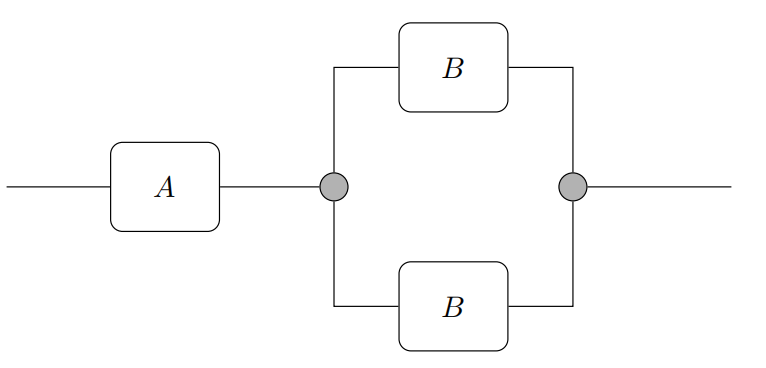
\includegraphics[scale=0.25]{system.png}
\end{center}
The system will fail if either component $A$ or both components marked $B$ fail. The components $A$ and $B$ have failure densities
$$
f_{A}(t)=\frac{1}{100} e^{-t / 100}
,
f_{B}(t)=\frac{1}{50} e^{-t / 50}, \quad t \geq 0
$$
respectively. What is the expected time of failure of the system?
\end{block}
\end{frame}

\begin{frame}{2. Misleading Bining}
\begin{center}
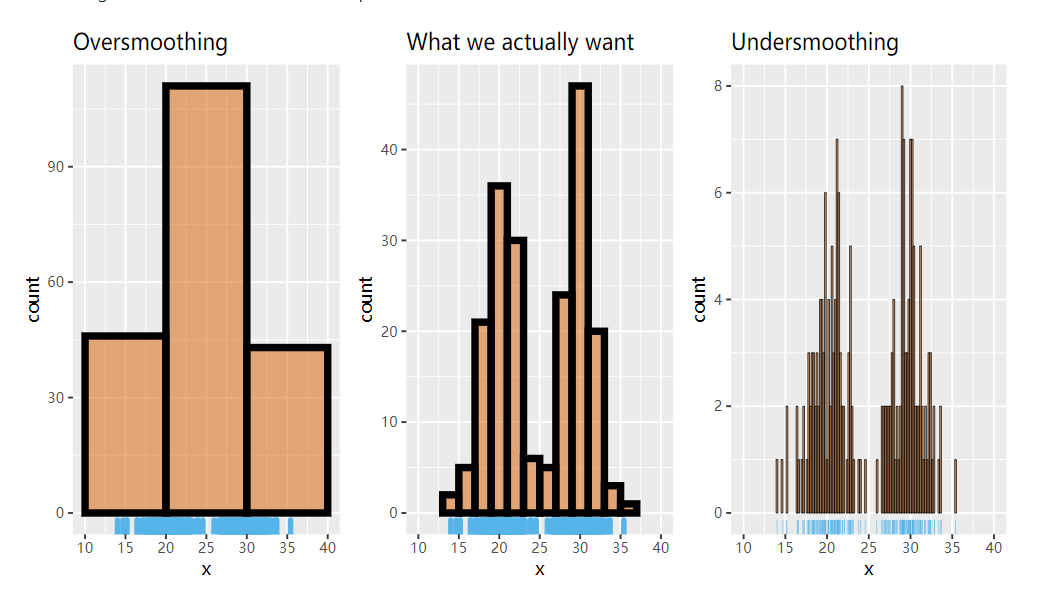
\includegraphics[scale=0.25]{mis1.png}

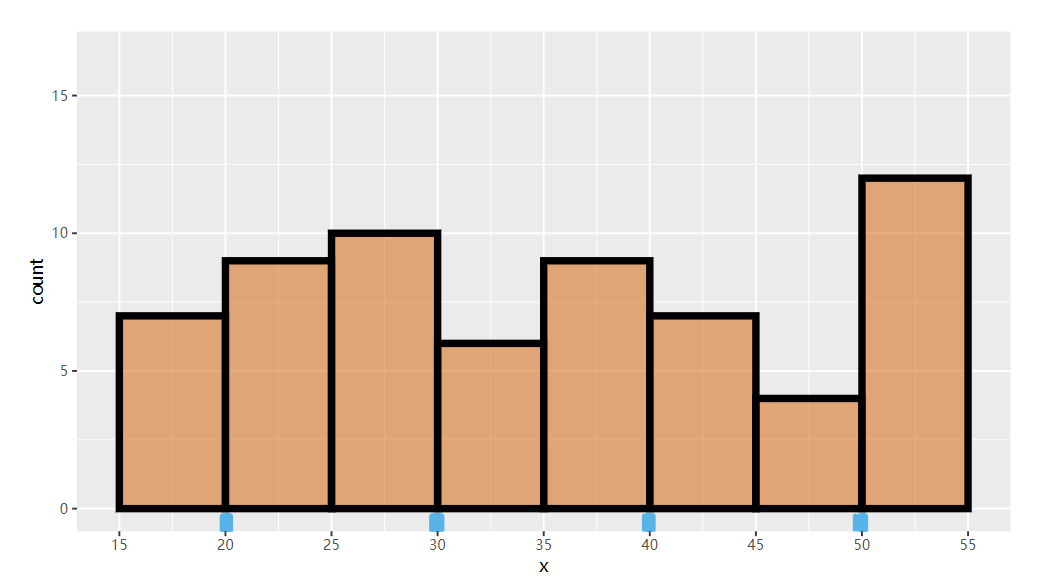
\includegraphics[scale=0.25]{mis2.png}
\end{center}
\tiny{\url{https://aakinshin.net/posts/misleading-histograms/}}
\end{frame}

\begin{frame}{3. Uniform Distribution Estimation}
\begin{block}{Exercise}
Estimator $\widehat{\Theta}$ is called an unbiased estimator for $\Theta$ if $E(\widehat{\Theta})=\Theta$ (notice that $\widehat{\Theta}$ is indeed a random variable!).
Consider a Uniform distribution on the interval $(0, \mathrm{~A})$.
\begin{itemize}
\item Is the maximum likelihood estimator for A unbiased?
\item Is $\widehat{A}_{1}=2 \widebar{X}_{n}$ an estimator for $\mathrm{A}$ ? Is it a reasonable estimator for $\mathrm{A}$ ? Is the above defined $\widehat{A}_{1}$ an unbiased estimator for A?
\item Is $\widehat{A}_{2}=2$ an estimator for $\mathrm{A}$ ? Is it a reasonable estimator for $\mathrm{A}$ ? Is the above defined $\widehat{A}_{2}$ an unbiased estimator for $\mathrm{A}$ ?
\end{itemize}
\end{block}

\end{frame}
\end{document}